\chapter{Review of Related Literature}

\section*{Time Series Analysis on hourly rainfall (Cutrim et al 2000)}

Time Series Analysis was used on an average hourly precipitation. The method determined whether statistically significant differences existed from each season. The data gathered is a 20-year period consisting of 2-hour intervals per day. In a seasonal analysis it was defined that winter, spring, summer, and fall are the seasons to be used. The Box-Jenkins methodology, a sample autocorrelation function (ACF) and a partial auto correlation function (PACF) plot were employed for each of the 12 periods of the day, for both precipitation accumulations and counts. A plot of ACF values at different lags was used to find a working series of stationary time points for the precipitation parameters accumulation and counts. For both precipitation parameters, the ACF plots clearly indicated the time series to be a non-seasonal component, but the same plot showed the need for further differencing of the seasonal component of the series, which occurs every four time periods. The periods of differencing, therefore, are 1 for the seasonal component of order 4. This differencing scheme produced a stationary time series, which is a prerequisite in ARIMA Modeling. 

The ACF and PACF plots of the differentiated series were then used to determine the autoregressive (AR) component and a moving average (MA) component of the series. Except for precipitation count at 6 a.m. the ARIMA model for cache of the differenced precipitation time series year were identified. (See Figure \eqref{newpic}).

\begin{figure}[!ht]
\centering
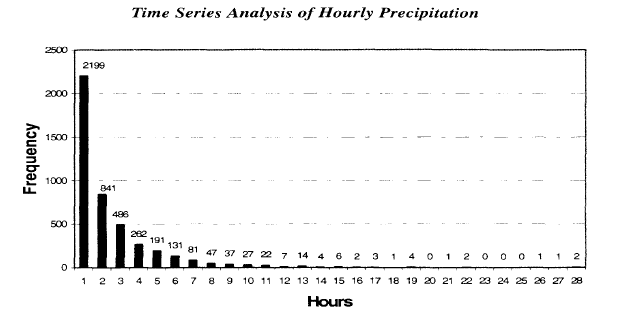
\includegraphics[width=4in, keepaspectratio]{daily}
\caption{\label{newpic} Time Series Analysis on a 50 year data of rainfall and temperature (Cutrim et al 2000).}
\end{figure}

A large set of data involving more than 50 years of rainfall and temperature data were examined using Spectral Analysis, Time Series Analysis-ARIMA Methodology to analyse climatic trends and interactions. Fourier analysis, linear regression and ARIMA based time series models were used to analyze the large data sets using Mat-lab, SPSS and SAS programs. The results that came up showed that the rainfall data was variable and appeared seasonal while the temperature data appeared stationary. Spectral analysis also showed variations in rainfall and temperature over 50-60 years but the results showed that rainfall and temperature varied coherently, with a cycle of about 2-3 years. An inverse relationship in trend was noted between rainfall and daily temperature range using linear regression among the variables. The ARIMA models showed autocorrelation and seasonality providing time series models.

It was concluded that: There is a cyclic pattern noted in both the rainfall and temperature time series and a cycle of about 3 years in the rainfall and temperature data sets suggesting a coherent variance in the relationship. This finding suggested a cyclic nature of large rainfall events over time and was confirmed by the recent large rainfalls events in 2009-10. Linear regression showed an inverse relationship in trend between rainfall and temperature range only even though the r value was around 0.27. 

\section*{Time Series Analysis on the Agricultural\\ Commodities Prices}

Other than prices, the data includes variables reflecting demand and supply factors affecting agricultural prices. Series are on a monthly basis. On the demand side it has been considered that monetary aggregate will be the proxy for world real aggregate expenditure, production of ethanol and biodiesel, several proxies for trading activity in futures markets, and the U.S. dollar–Euro exchange rate. On the supply side the price of oil, price of fertilizers, and volume of exports by major world producers are used. 

The data gathered was from 2002 to 2009. The end of the series was restricted due to unavailable data, and restrictions at the beginning of the series were due to the presence of structural changes based on Chow tests. All price data and other variables will be taken in log form when analyzed.

\section*{The distribution of monthly rainfall}

Monthly distributions of rainfall in space and time can provide guidelines for crop scheduling and for introducing better cropping patterns in the region.

To determine the periodicity of the monthly rainfall sequence at a station, the method developed by Vujica M. Yevjevich was used, in which the parameters involved are clearly defined. 

It was found that monthly rainfall sequences at all the stations under consideration
have six significant harmonics, which means that the monthly rainfall has a periodic part that consists of components corresponding to the following six periods: 12, 6, 4, 3, 2.4 and 2 months. The variances of the monthly means and the monthly standard deviations are explained up to more than 90\%  by these six significant harmonics. These findings show that after removing the first six periodic components, the residual rainfall sequence at a station can be considered to be stationary at least in the mean and standard deviation. (See Table 1.)

For most cases, the serial correlation coefficient between two successive monthly
rainfall sequences at a station were found not to be significantly different from zero. Nonsignificance of correlation does not necessarily imply statistical independence, monthly rainfall totals were analysed separately and a probability distribution was fitted month by month.

\begin{table}
\centering
\begin{tabular}{ccc}
\toprule
Station & Mean & Standard Deviation\\
\midrule
Buriram & 0.925 & 0.917\\
Chaiyaphum & 0.940 & 0.938\\
Kalasin & 0.924 & 0.920\\
Khon Kaen & 0.927 & 0.937\\
Loei & 0.924 & 0.921\\
Maha Sarakham & 0.935 & 0.921\\
Nakhon Phanom & 0.924 & 0.979\\
Nakhon Ratchasima & 0.931 & 0.920\\
Nongkhai & 0.919 & 0.929\\
Roi Et & 0.922 & 0.919\\
Sakhon Nakhon & 0.917 & 0.941\\
Ubon Ratchatani & 0.922 & 0.942\\
Udon Thani & 0.917 & 0.927\\
Yasothon & 0.927 & 0.939\\
\bottomrule
\end{tabular}
\caption{\label{tab:first} The residual rainfall sequence in agricultural provinces in Thailand.}
\end{table}

It was concluded that each monthly rainfall sequence has a periodic part consisting of six constituents corresponding to the following six periods: 12, 6. 4, 3, 2.4 and 2 months.
At each station the rainfall sequence in a month is independent of the rainfall sequences in the other months. Since many monthly rainfall sequences in the Northeast have zero values, the leakage law is most appropriate for fitting these sequences. Monthly rainfall in the region varies greatly from month to month, resulting in high degrees of irregularity, ranging from 45 to 70 per cent. Monthly rainfall also varies greatly from year to year as indicated by the high values for the coefficient of variation. The eastern and north-eastern sections of the region are the wettest areas of the Northeast from April to September but they are the driest parts from October to December. The maximum amount of rainfall for the entire region usually occurs in August or September while the minimum normally occurs in December or January.